\subsection{MDP-Tetris}

When running the experiments, the source code of the MDP-Tetris
\citep{mdptetris} was used to emulate the Tetris games.
The source code is accompanied with files that describe the
various existing features. These files contains the identifiers of 
each feature to use, as well as two numbers respectively describing 
the agents reward function and how to evaluate a game over state. 
The number for the reward function has remained unchanged at $0$ 
during all experiments. The "game-over" evaluation was for the
Bertsekas feature set initially set to $0$. Setting the 
"game-over" evaluation to $0$ means that the agent will not 
distinguish between regular moves and moves that results in losing
the game. When running the experiments with this setting, a large portion
of the agents never exceeded a zero mean score. However, setting the value
to $-1$, meaning that a "game-over" move yields $-\infty$ reward, 
none of the experiments got stuck on only zero scores. An example
of the layout of the feature file can be seen in figure \ref{fig:featfile}.
\begin{figure}[h!]
\centering
\begin{lstlisting}
0    <- Describes the reward function
-1   <- Actions leading to game over is avoided at all cost
22   <- The policy contains 22 features
8 0  <- The feature with id 8 initially has weight 0
...  <- The remaining 21 features
\end{lstlisting}
\caption{Example of a file that describes a feature set. \label{fig:featfile}}
\end{figure}

\subsubsection{Featureset}

As described in \comment{Theory section ref}, there are different kind of featuresets which
impacts the performance of the agents. In our upcoming experiments, we are going to
use both the Dellacherie and Bertsekas/Tsitsiklis featureset. For our initial comparison experiments
we are going to use the Bertsekas/Tsitsiklis featureset, since other researchers report
a lower score with the Bertsekas/Tsitsiklis featureset compared with the Dellacherie featureset
\citep{thiery:09}. Compared to the \citep{thiery:09} experiments, we don't want to maximize the
final score, but rather maximize the score with the lowest possible number of 
games evaluated.\\
It's important to note that we are not going to conduct comparison experiments with different
featuresets in the same experiment, since the algorithms needs to be on equal terms.

\subsubsection{Game complexity \label{HardTetris}}

\begin{table}[H]
\centering
\small
\begin{tabular}{c c c r r r r}
Tetris Type & Optimizer & mean & Q1 & Q2 & Q3\\
\hline
Hard & Cross Entropy & $1633.607$ & $1357.170$ & $1606.565$ & $1938.71$\\
Normal & Cross Entropy & $100059.463$ & $79357.440$ & $105999.500$ & $111047.500$\\
Hard & CMA & $449.352$ & $201.850$ & $300.300$ & $529.350$\\
Normal & CMA & $49760.161$ & $42528.740$ & $49915.700$ & $67764.729$\\
\end{tabular}
\caption{Experiment testing game Normal Tetris against Hard Tetris}
\end{table}

\begin{figure}[H]
\centering
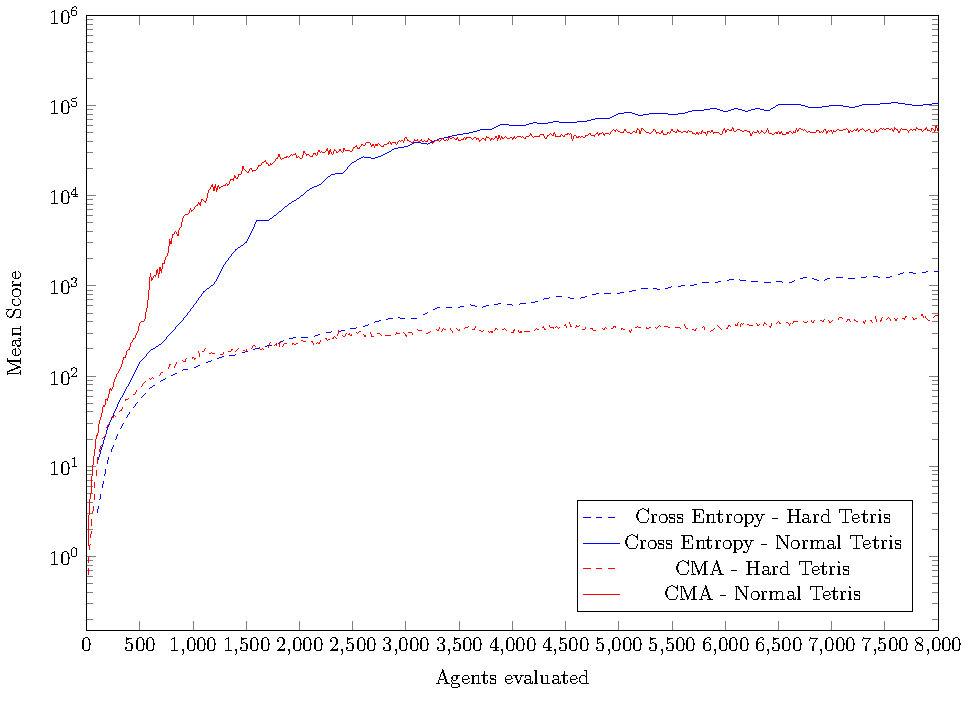
\includegraphics[scale=1]{data/complexity/mean/PlotFile.pdf}
\caption{Experiment testing game Normal Tetris against Hard Tetris}
\end{figure}

\comment{- Write stuff aboutGame complexity and the difference it can make}\\

\comment{- The stuff about hard tetris in the comparison section should be here?
This probably requires some restructuring of the report to make sense. For example 
we conclude in the featureset comparison section that we are going to use hard tetris
for configuration of CMA, which doesn't make sense, since CMA "already" has been configured 
at this point.}



